\documentclass{beamer}
\usepackage[T1]{fontenc}
\usepackage[utf8]{inputenc}
\usepackage{lmodern}
\usepackage{graphicx}
\usepackage[absolute,overlay]{textpos}
\usepackage{multicol}
\usepackage{listings}
\usepackage{svg}

%% Beamer customization--------------------------------------------------------

\usepackage{xcolor}


%% Define Snakemake -----------------------------------------------------------

\definecolor{eclipseBlue}{RGB}{42,0.0,255}
\definecolor{eclipseGreen}{RGB}{63,127,95}
\definecolor{eclipsePurple}{RGB}{127,0,85}

\lstset{language=Python}
\lstset{
    basicstyle=\scriptsize\ttfamily,
    morekeywords={rule, output, shell, params, run, configfile, temp, log},
    showstringspaces=false,
    commentstyle=\color{eclipseGreen}, % style of comments
    keywordstyle=\color{eclipsePurple}, % style of keywords
    stringstyle=\color{eclipseBlue}, % style of strings
}



\usepackage{tikz}

\usetheme{Warsaw}

%% Themes
% Outer themes
\useoutertheme{shadow}
% Rounded boxes and shadows
\useinnertheme[shadow=true]{rounded}
% Solid \item symbols
\useinnertheme{circles}

%% Custom colors
\definecolor{rltgreen}{rgb}{0,0.5,0}
\definecolor{pasteur}{RGB}{0,90,154}
\setbeamerfont{block title}{size={}}
\setbeamercolor{structure}{fg=pasteur}
\setbeamercolor{item}{fg=pasteur}


%Color of title
\setbeamertemplate{frametitle}
{    \nointerlineskip
    \begin{beamercolorbox}[sep=0.3cm,ht=1.8em,wd=\paperwidth]{frametitle}
        \vbox{}\vskip-2ex%
        \strut\insertframetitle\strut
        \vskip-0.8ex%
    \end{beamercolorbox}
}
% Hide navigation symbols
\setbeamertemplate{navigation symbols}{}

%% Title block
\setbeamercolor*{title}{use=structure,fg=white,bg=pasteur}

\makeatletter

%% Top infolines
\setbeamertemplate{headline}{%
\leavevmode%
  \hbox{%
    \begin{beamercolorbox}[wd=\paperwidth,ht=2.5ex,dp=1.125ex]{palette quaternary}%
    \insertsectionnavigationhorizontal{\paperwidth}{}{\hskip0pt plus1filll}
    \end{beamercolorbox}%
  }
}



\title[Sequana]{Sequanix: A Dynamic Graphical Interface for Snakemake Workflows}
\author[T. Cokelaer]{Thomas Cokelaer, Dimitri Desvillechabrol, Rachel Legendre, 
Christiane Bouchier, Sean Kennedy}
\institute{Institut Pasteur, Paris}
\date{July 4th 2017, JOBIM 2017, Lille}


\AtBeginSection[]{
  \begin{frame}
  \vfill
  \centering
  \begin{beamercolorbox}[sep=8pt,center,shadow=true,rounded=true]{title}
    \usebeamerfont{title}\insertsectionhead\par%
  \end{beamercolorbox}
  \vfill
  \end{frame}
}

\begin{document}

%% Title slide ----------------------------------------------------------------

\begin{frame}[plain]
    \titlepage
    \begin{textblock*}{5cm}(4.5cm,0.3cm)
        
\includegraphics[scale=0.09]{images/Institut_Pasteur.png}
    \end{textblock*}
\end{frame}



%\usebackgroundtemplate{\centering
%\includegraphics[width=\paperwidth,
%height=\paperheight]{images/strand.png}}

%\addtobeamertemplate{block 
%begin}{\pgfsetfillopacity{0.5}}{\pgfsetfillopacity{1}}
%\addtobeamertemplate{block alerted 
%begin}{\pgfsetfillopacity{0.5}}{\pgfsetfillopacity{1}}
%\addtobeamertemplate{block example 
%begin}{\pgfsetfillopacity{0.5}}{\pgfsetfillopacity{1}}


%% Slides ---------------------------------------------------------------------

\begin{frame}
\frametitle{Motivation}
\begin{block}{Provide NGS pipelines @ Biomics sequencing platform 
https://research.pasteur.fr/en/team/biomics/ (Institut Pasteur)}
 \begin{itemize}
  \item Genomics: QC + variant calling + de-novo
  \item Transcriptomics: RNA-seq + ChIP-seq 
  \item Metagenomics
  \item Illumina but also Pacbio long reads technologies
 \end{itemize}
 %\includegraphics{images/genetic_strand.png}
 %\includegraphics{images/strand.png}
\end{block} 
\end{frame}

\usebackgroundtemplate{}

\begin{frame}
\frametitle{How ?}

\begin{columns}
\begin{column}{1.5cm}

\includegraphics[height=0.2\textheight]{images/logo_python.png} 
\end{column}
\begin{column}{9cm}
a glue language, a scientific language
\end{column}
\end{columns}

\rule{\textwidth}{1pt}


\begin{columns}
\begin{column}{1.5cm}

\includegraphics[height=0.2\textheight]{images/logo_snakemake.png}
\end{column}
\begin{column}{9cm}
a pipeline 
framework mixing Python and Makefile \\
{\footnotesize \textcolor{blue}{\textit{Köster, Johannes and Rahmann, Sven. 
Snakemake - A scalable 
bioinformatics workflow engine. Bioinformatics 2012.}}}
\end{column}
\end{columns}

\rule{\textwidth}{1pt}


\begin{columns}
\begin{column}{1.5cm}

\includegraphics[height=0.2\textheight]{images/exe.png}
\end{column}
\begin{column}{9cm}
Dedicated standalone such as genome coverage characterisation.\\
{\footnotesize \textcolor{blue}{\textit{D. Desvillechabrol, C. 
Bouchier, S. Kennedy, T. Cokelaer Detection and characterization of low 
and high genome coverage regions .... BioRxiv 
https://doi.org/10.1101/092478 }}}
\end{column}
\end{columns}
\end{frame}



\begin{frame}
\frametitle{How ? Sequana}
\vspace{2cm}

$\begin{array}{l}

\includegraphics[height=0.18\textheight]{images/logo_python.png}
\end{array}$
{\Huge +}
$\begin{array}{l}

\includegraphics[height=0.18\textheight]{images/logo_snakemake.png}
\end{array}$
{\Huge +}
$\begin{array}{l}

\includegraphics[height=0.18\textheight]{images/exe.png}
\end{array}$
{\LARGE = Sequana}

\centering
\vspace{2cm}
\Large
http://sequana.readthedocs.io

\end{frame}

\begin{frame}
\frametitle{Pipeline example 1: Sequana quality control pipeline} 
\centering
 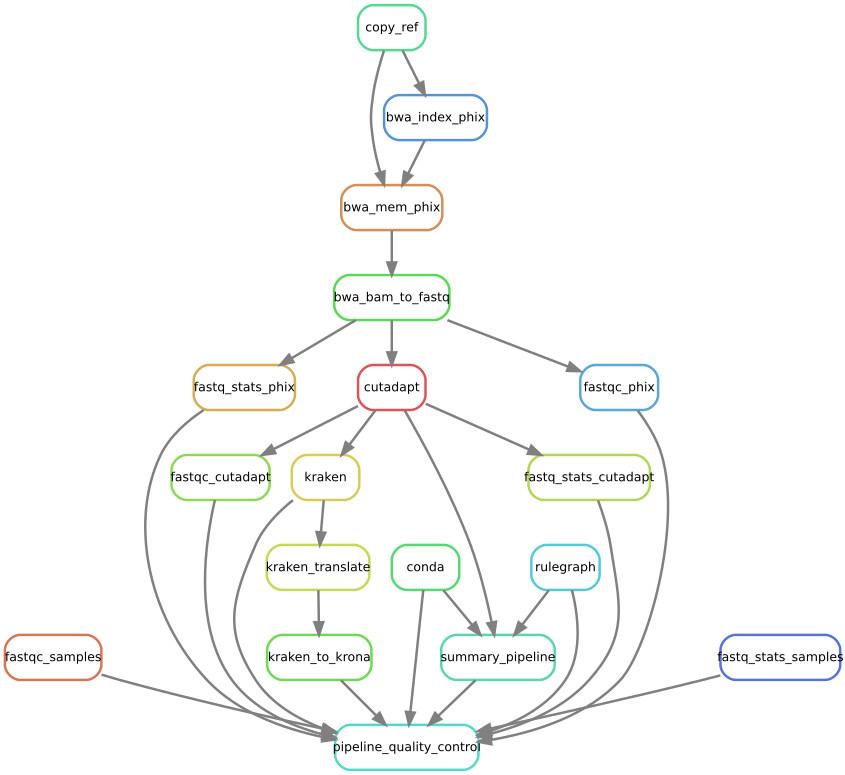
\includegraphics[height=0.8\textheight, width=\textwidth]{./images/dag_qc.png}
\end{frame}

\begin{frame}[fragile]
\frametitle{Pipeline example 2: minimalist (GC content)} 
\centering

\begin{columns}
 \begin{column}{7.2cm}
 \hspace{-2cm}
\begin{lstlisting}
# list of FastQ files without extension
files = ["A", "B", ....]

rule all:
    input: expand("{data}.png", data=files), 
        "index.html"

rule create_GC_images:
    input: "{data}.fastq.gz"
    output: "{data}.png"
    run: # CODE TO COMPUTE IMAGES
        
rule html_report:
    input: expand("{data}.png", data=files)
    output: "index.html"
    run: # CODE TO CREATE HTML 
\end{lstlisting} 
\end{column}
\begin{column}{3.9cm}
\hspace{1cm}
 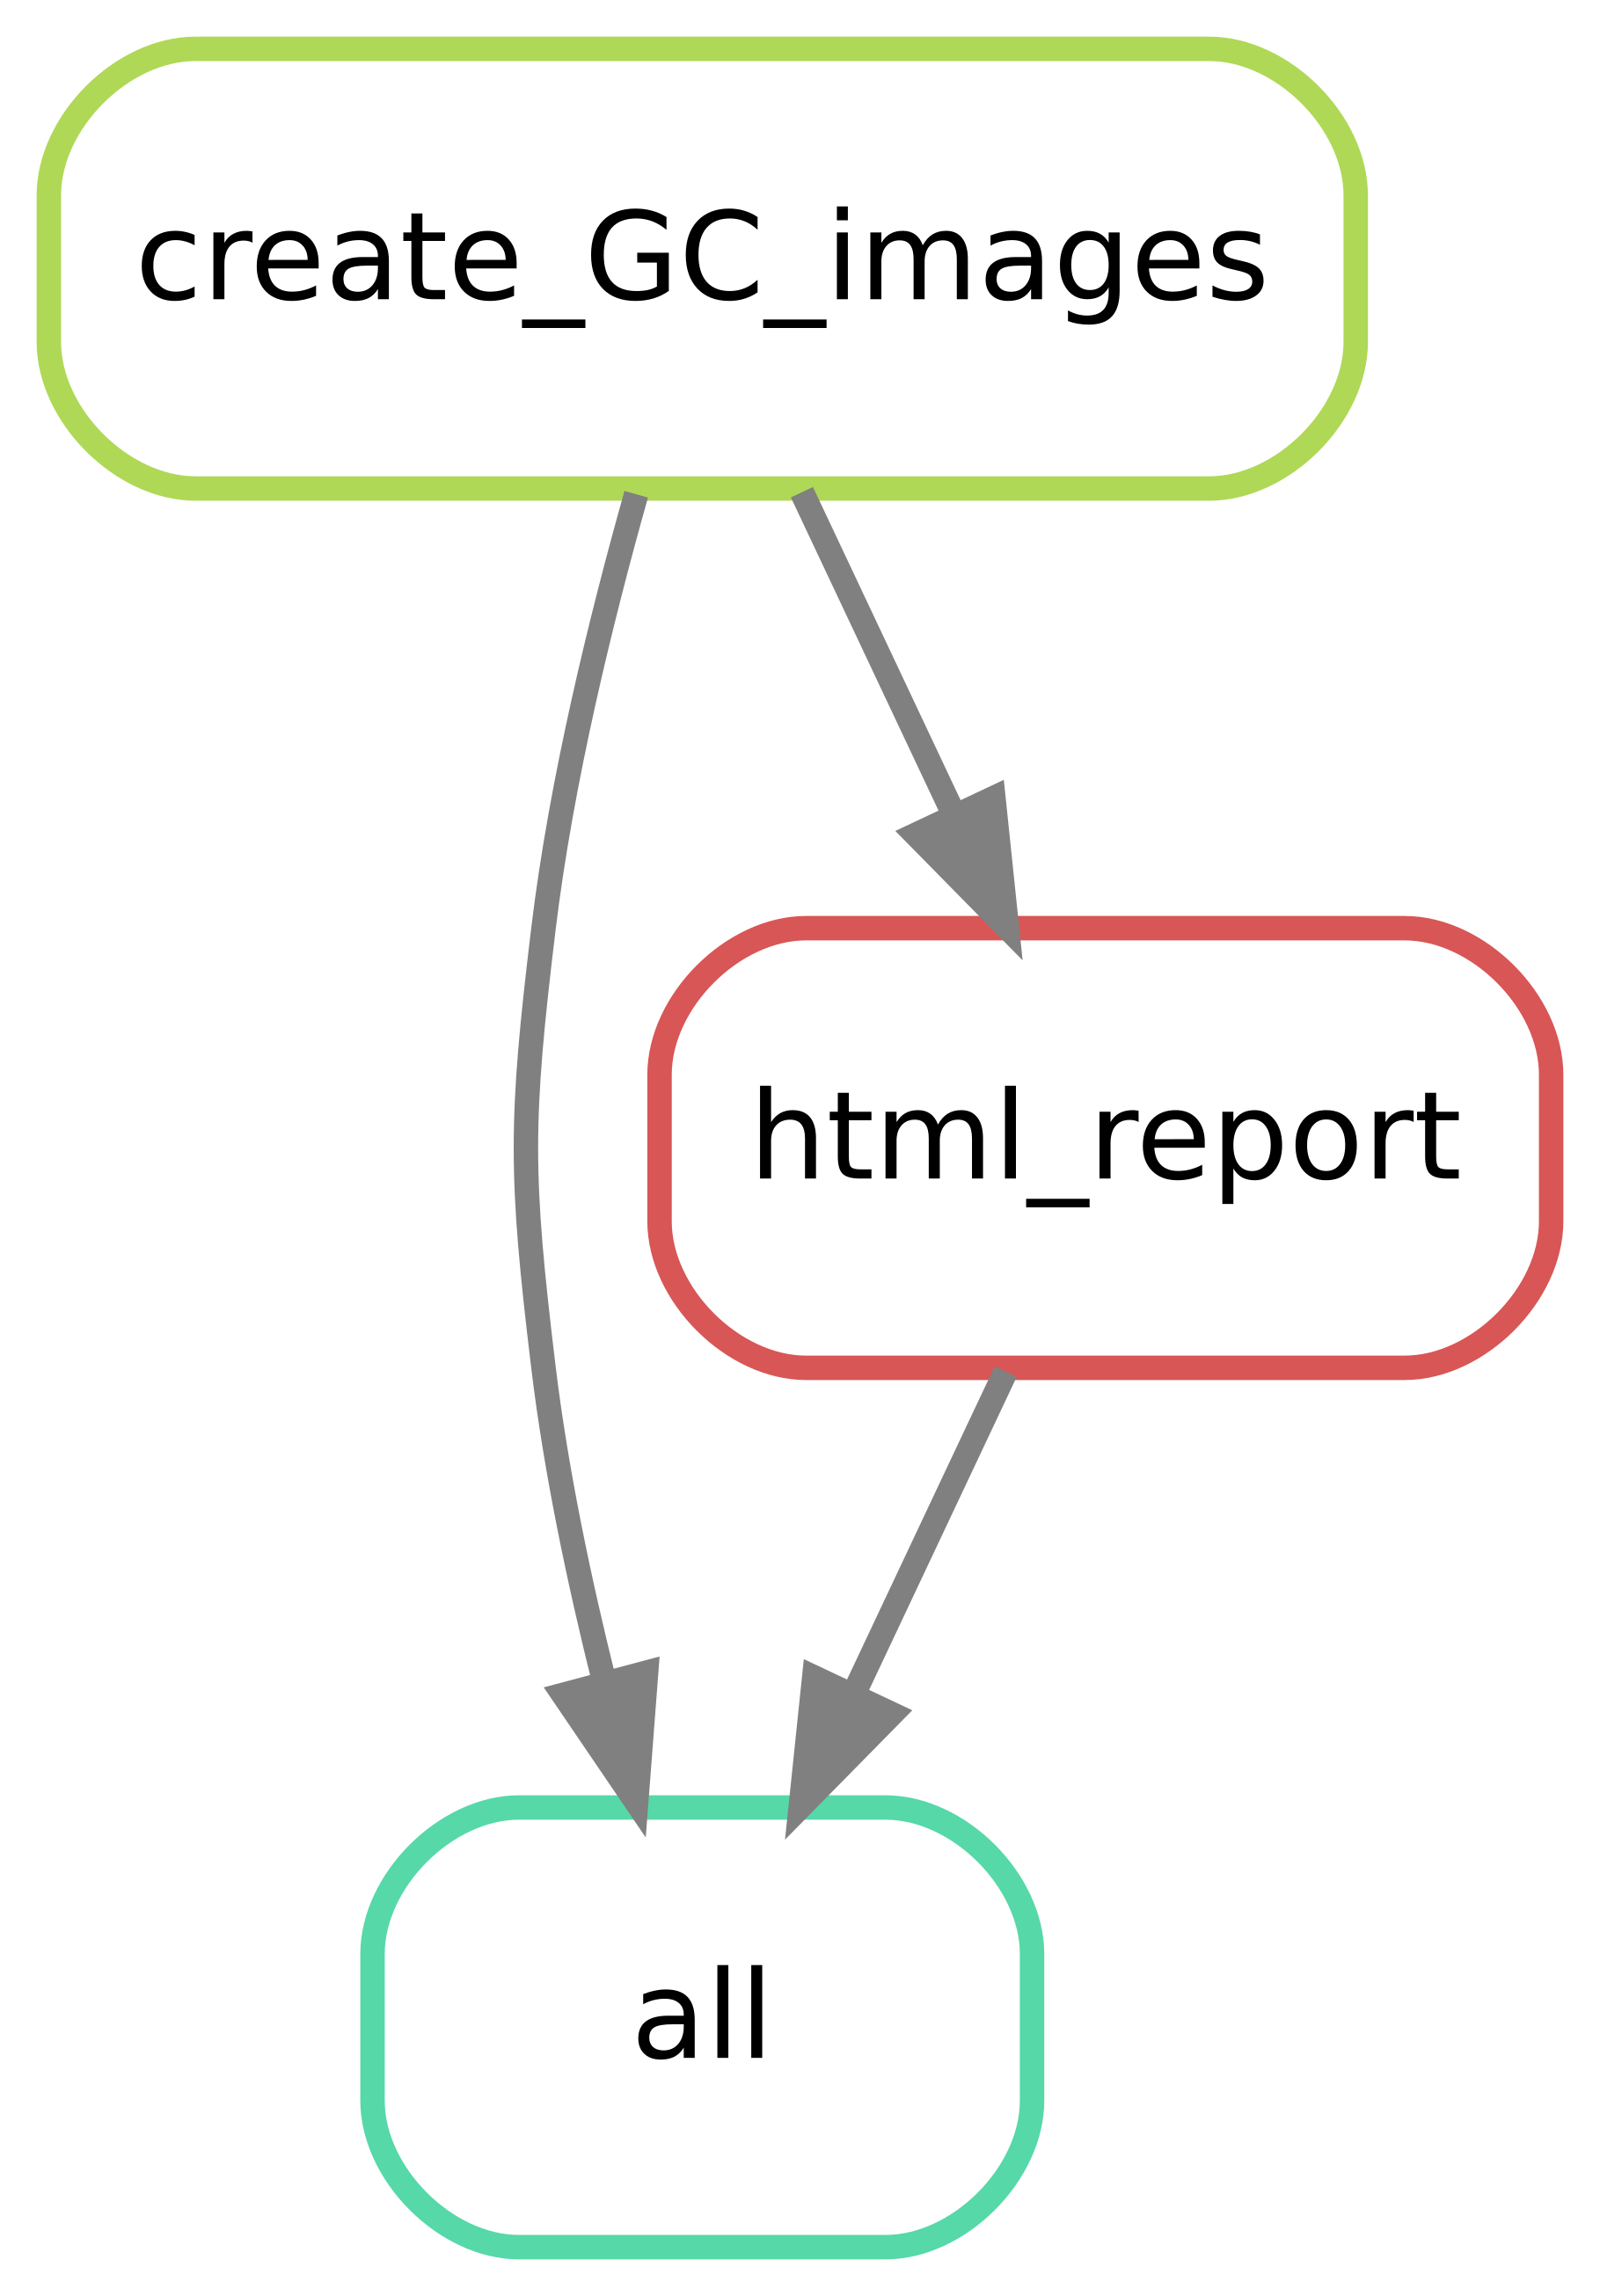
\includegraphics[scale=2.2]{./images/gc.png}
\end{column}
\end{columns}
\end{frame}


\begin{frame}[fragile]
\begin{block}{configuration file example in YAML format}
 \begin{lstlisting}
##########################################################
# Input parameters for the fractal analysis
#
# :Parameters: 
#
# - size: output image size formatted as NxM where N and M 
#         are integers
# - depth: a integer (e.g. 200)
# - zoom: a positive value e.g. 0.5
# - N: number of random sets
gc_content:
    - window: 100
    - directory: /home/user/fastq_files
    - recursive: false
 \end{lstlisting}
\end{block}
\end{frame}


\begin{frame}[fragile]
\frametitle{Execution}

From a shell:
\rule{\textwidth}{1pt}


\begin{lstlisting}[basicstyle=\ttfamily\large]
snakemake -s gc_minimalist.rules
\end{lstlisting}

\rule{\textwidth}{1pt}

More options if a configuration file is required, or execution is on a cluster, 
or \dots something goes wrong.
\end{frame}


\section{What about a GUI interface ?}
\begin{frame}
\frametitle{Sequanix: a standalone application in PyQt}

\begin{block}{Sequanix}
\begin{itemize}
 \item Users do not want to see the Snakefile
 \item Developers do not want users to see the Snakefile
 \pause
 \item Users do not want to edit the configuration file manually
 \item Developers do not want users to edit the configuration file manually
 \pause
 \item We want a GUI that works on a local computer or on clusters.
 \pause
 \item Sequana developers want to expose their pipelines dynamically
 \pause
 \item Snakemake developers want to use Sequanix ;-) 
\end{itemize}
\end{block}
\end{frame}



\section{DEMO}



\begin{frame}
\frametitle{Sequanix is part of Sequana project}
\centering

\includegraphics[scale=0.3, height=7cm]{images/logo.png}

\end{frame}

\begin{frame}

\begin{block}{You like it?}
 Try it: it is on Bioconda (conda install sequana)
\end{block}

\begin{block}{Questions ?}
Tomorrow's poster session at 11.45: number 93
\end{block}

\end{frame}

\begin{frame}
\frametitle{Merci gramint à vouzotes}
Thank you to the members of the bioinformatics and biostatistics HUB of 
Institut Pasteur (C3BI) as well as  Claire Roualen and Jacques van Helden for useful 
discussions.


\end{frame}






\end{document}
